% $Id: UMLRef.tex,v 1.1 2008/01/31 18:04:17 dconway Exp $
\chapter{\label{chapter:UMLDiagrams}Unified Modeling Language (UML) Diagram Notation}
\chapauthor{Darrel J. Conway}{Thinking Systems, Inc.}

This appendix presents an overview of the Unified Modeling Language diagrams used throughout the
text, including mention of non-standard notations in the presentation.  A more thorough presentation
is given in \cite{fowler}.

The presentation made here uses UML to sketch out how GMAT implements specific components of the
architecture.  What that means is that the UML diagrams in the text do not necessarily present the
full implementation details for a given system component.

All of the UML diagrams in this document were drawn using Poseidon for UML, Professional edition
\cite{poseidon}.  The compressed UML files for these diagrams are configuration managed in a
repository at Thinking Systems' home office.

\section{Package Diagrams}

\begin{figure}[htb]
\begin{center}
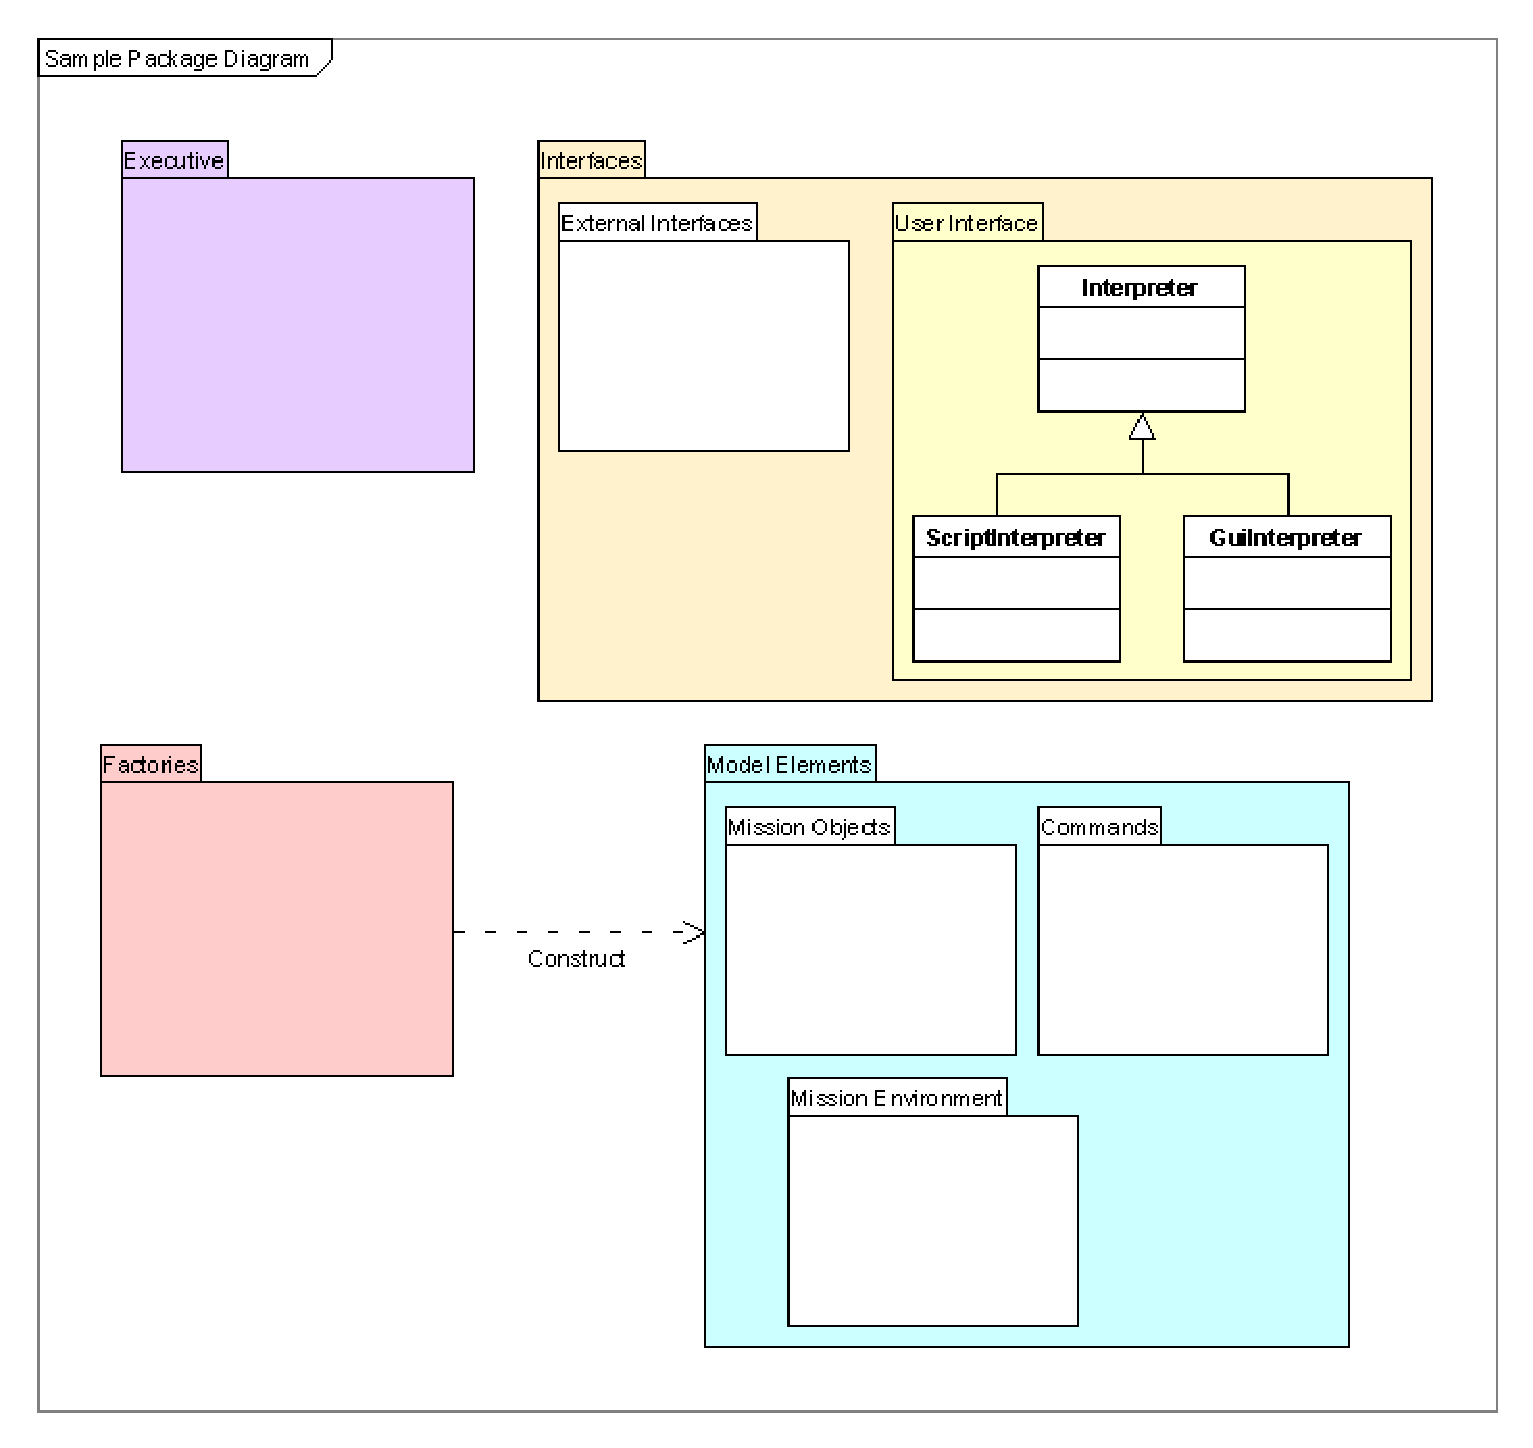
\includegraphics[scale=0.5]{Images/UmlPackageSample.eps}
\caption{\label{figure:UmlPackageExample}GMAT Packaging, Showing Some Subpackaging}
\end{center}
\end{figure}

Package diagrams are used to present an overview of a collection of objects, ranging from the top
level parts of an entire system to subelements of subsystems.  Figure~\ref{figure:UmlPackageExample}
shows an example of a
package diagram.  In this figure, four primary GMAT system subsystems are shown: the Executive
subsystem, the Interfaces, the Factory subsystem, and the model elements.

Each box on the diagram represents a group of one or more classes that perform a task being
discussed.  Package diagrams may include both package boxes and class boxes.  The packages are
represented by a box with a tab on the upper left corner; classes are represented by boxes which may
be subdivided into three regions, as described in the Class Diagram section.  Packages can be
further divided into constituent elements, either subpackages within a given package, or classes in
the package.  For example, in the figure, the interface package consists of an External Interface
package and a User Interface package.  The User Interface package is further broken into three
classes: the Interpreter base class and the ScriptInterpreter and GuiInterpreter derived classes.

Sometimes important interactions are included in the Package diagram.  When this happens, the
interaction is drawn as a dashed arrow connecting two elements on the diagram, and the nature of the
interaction is labeled.  In the example, the relationship between the Factory package and the Model
Element package is included: Factories are used to construct model elements.

In this document, package diagrams are used to communicate design structure.  The packages shown in
the figures do not explicitly specify namespaces used in the GMAT code, even though UML does allow
that use for package diagrams.  When a package documented here has implications for a namespace used
in GMAT, that implication will be explicitly presented in the accompanying text.

\section{Class Diagrams}

\begin{figure}[htb!]
\begin{center}
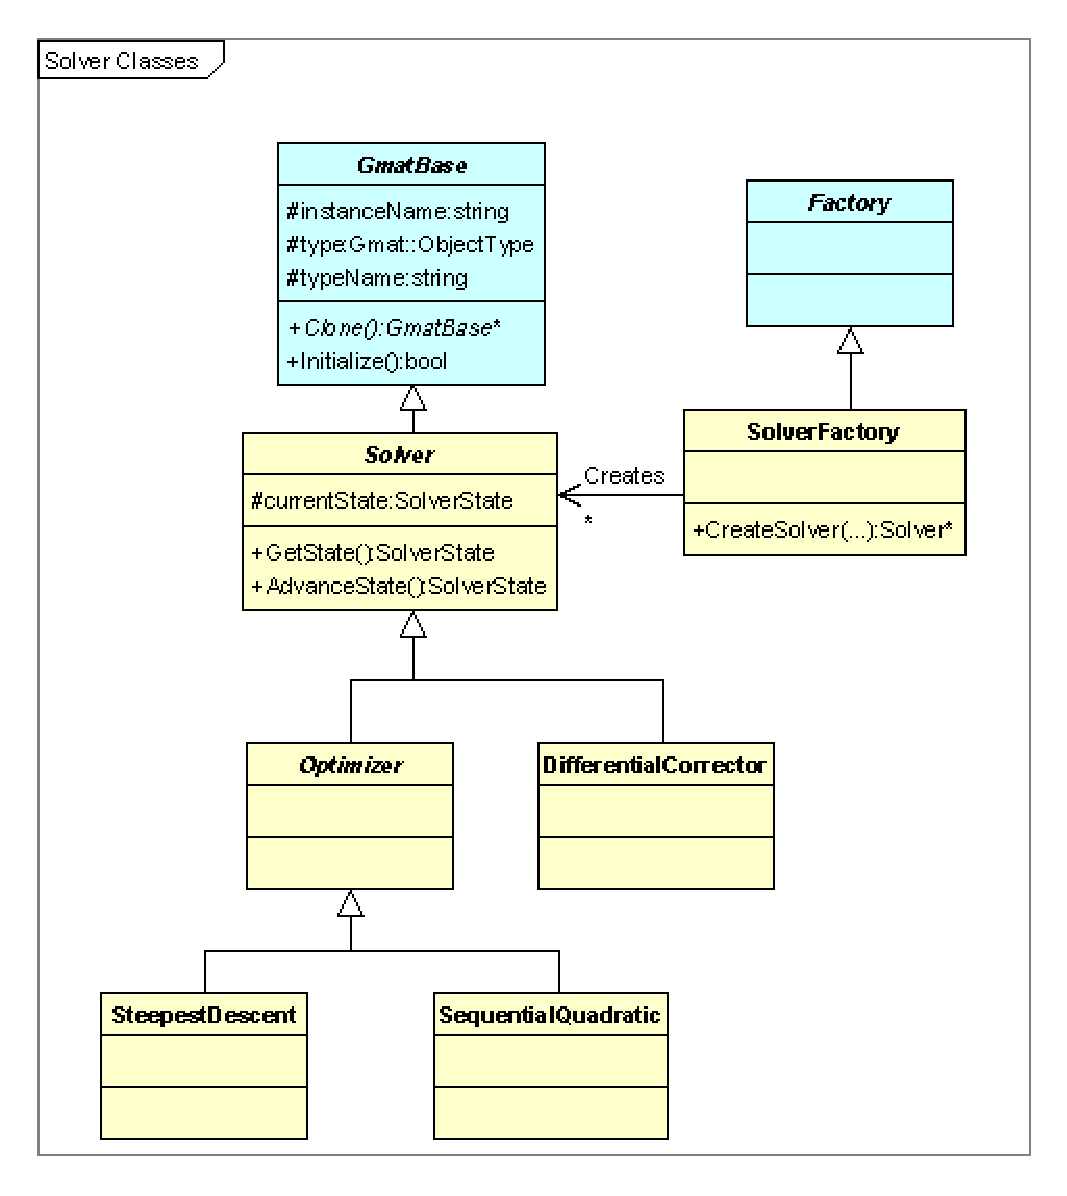
\includegraphics[scale=0.5]{Images/UmlClassSample.eps}
\caption{\label{figure:UmlClassExample}Solver Classes}
\end{center}
\end{figure}

Figure~\ref{figure:UmlClassExample} shows a typical class diagram for this document.  This figure is
an early version of the class diagram for the solver subsystem.  The classes directly used in that
subsystem are colored differently from the related base classes -- in this figure, the Solver
classes have a yellow background, while the base classes are blue.  Each box on the diagram denotes
a separate class; in this example, the classes are GmatBase, Solver, Optimizer, SteepestDescent (removed in R2019a),
SequentialQuadratic, DifferentialCorrector, Factory, and SolverFactory.  Abstract classes are
denoted by italicizing the class name; here the classes GmatBase, Solver, Optimizer, and Factory are
all abstract because they contain pure virtual methods.

The box representing the class is broken into three pieces.  The top section indicates the name of
the class.  The center section lists the attributes (i.e. data members) of the class, and the bottom
section stores the operations (aka methods) available for the class.  Attributes and operations are
prefaced by a symbol indicating the accessibility of the class member; a `+' prefix indicates that
the member is publicly accessible, `\#' indicates protected access, and `-' indicates private
access.  Static members of the classes are underlined, and singleton classes receive a
$<<$Singleton$>>$ designation above the class name.

The class diagrams included in this document suppress the argument list for the methods.  This is
done for brevity's sake; the model files include the argument lists, as does the code itself, of
course.  When a method requires arguments, that requirement is indicated by ellipses on the diagram.

Classes are connected to one another using lines with arrows.  If the arrowhead for the line is a
three-sided triangle, the line indicates inheritance, with the line pointing from the derived class
to its base.  For example, in the figure, SolverFactory is derived from the Factory base class. 
SolverFactory is not abstract, and can be instantiated, but Factory is an abstract class as
represented in this figure (the class name is italicized), even though the figure does not
explicitly provide a reason for the class to be abstract.

Lines terminated by an open arrowhead, like the line connecting SolverFactory to the Solver base
class, indicates an association.  The arrow points in the direction that the association is applied
-- in this case, the SolverFactory creates instances of Solvers.  The decorations at the ends of
these lines indicates multiplicity.  An asterisk indicates 0 or more, so for this example, a
SolverFactory can create 0 or more Solvers, depending on the needs of the program during execution.

\section{Sequence Diagrams}

\begin{figure}[htb]
\begin{center}
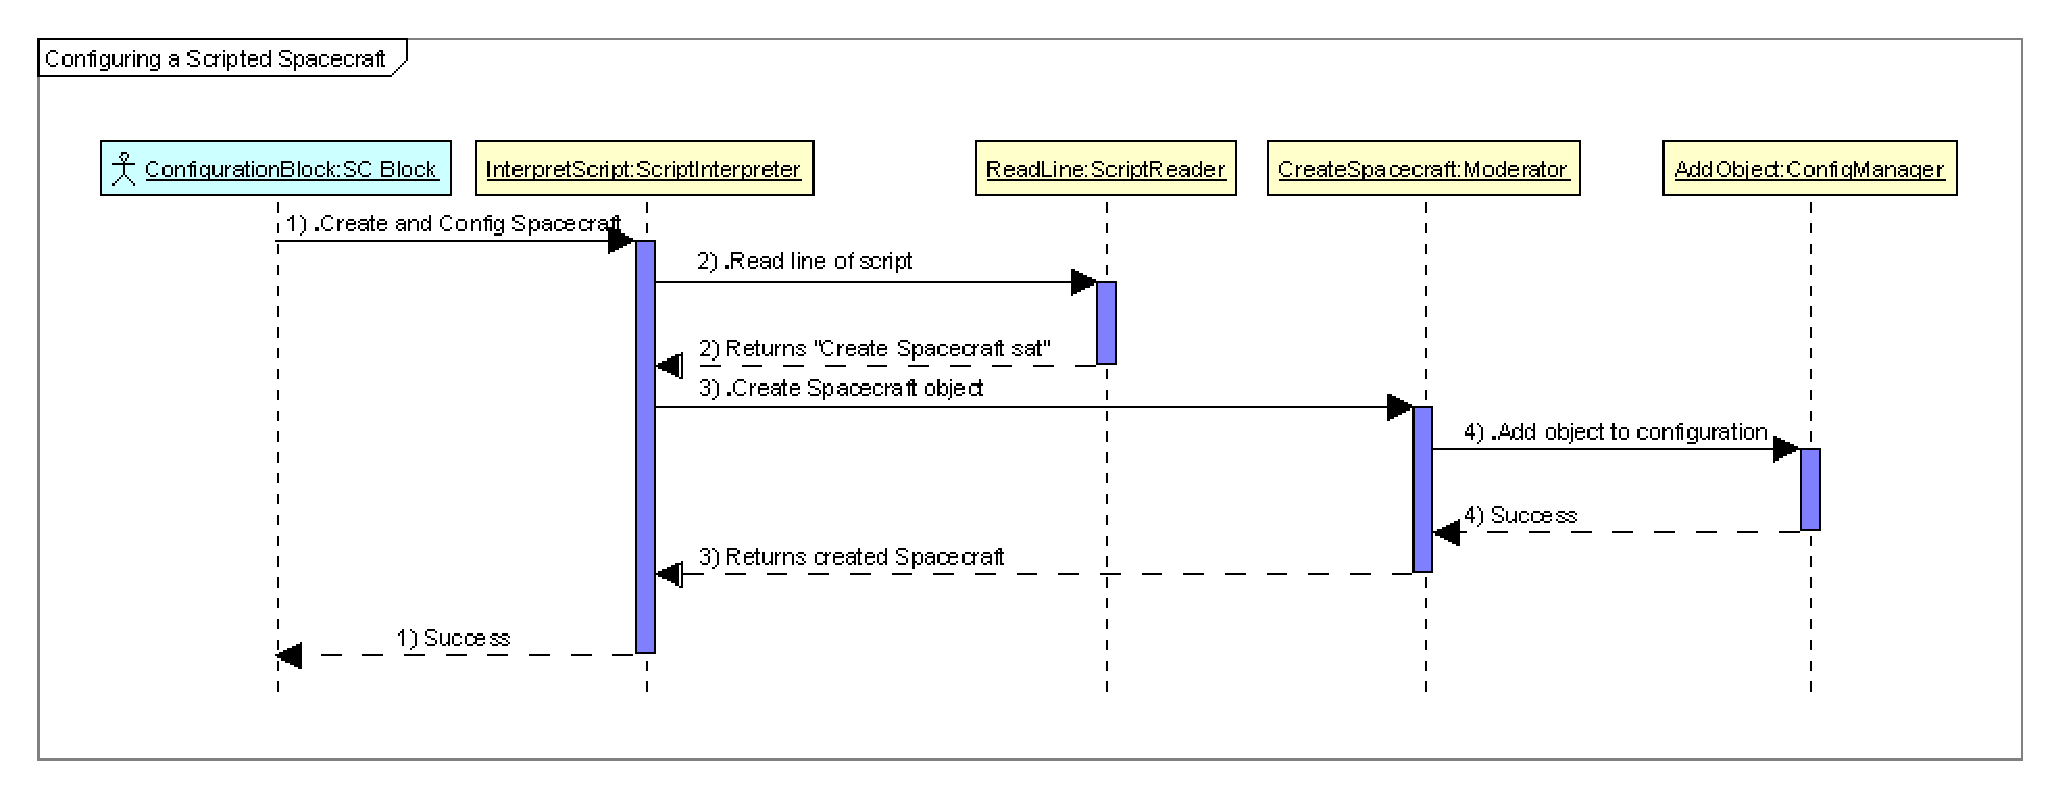
\includegraphics[scale=0.45]{Images/UmlSequenceSample.eps}
\caption{\label{figure:UmlSequenceExample}A Sequence Diagram}
\end{center}
\end{figure}

Sequence Diagrams are used to indicate the sequence of events followed when performing a task.  The
task shown in Figure~\ref{figure:UmlSequenceExample} is the creation of an instance of the
Spacecraft class from the ScriptInterpreter.  Sequence diagrams are used in this document to
illustrate a time ordered sequence of interactions taken in the GMAT code.  In this example, the
interactions between the ScriptInterpreter and the other elements of GMAT are shown when a "Create
Spacecraft..." line of script is parsed to create a Spacecraft object.

Each of the players in the illustrated action receive a separate timeline on the figure, referred to
as a ``lifeline''.  Time flows from top to bottom.  The player is described in the label at the top
of the lifeline.  In the example shown here, each player is a method call on a core GMAT object --
for example, the line labeled CreateSpacecraft:Moderator represents the
Moderator::CreateSpacecraft(...) method.  Sequence diagrams in this document can also use lifelines
to for larger entities -- for instance, the sequence diagram that illustrates the interaction
between the GUI, ConfigManager, Moderator, Sandbox, and mission components when a mission is run,
Figure~\ref{figure:RunningBasicScript}.  The vertical blocks on each lifeline indicate the periods
in which the lifeline is active, either because it is being executed, or because it is waiting for a
called method to return.

Blocks are nested to indicate when a function is called inside of another.  In the example, the
ConfigManager::AddObject(...) call is nested inside of the Moderator::CreateSpacecraft(...) call
because that inner call is performed before control returns from the Moderator function.  Arrows
from one lifeline to another are used to indicate the action that is being performed -- in the
example, line 4 shows when the newly created Spacecraft is handed to the Config manager.  (Note that
this is a bit more verbose than in the UML standard; the standard is to just list the method that is
called, while I prefer to give a bit more description of the invoked operation.)

Iteration can be indicated on these diagrams by enclosing the iterated piece in a comment frame. 
Similarly, recursion is indicated by a control line that loops back to the calling timeline.  When
this type of action occurs, a note is also included on the figure to indicate how the recursion or
self reference gets resolved; an example can be seen in Figure~\ref{figure:ParserRecursion}.  (These
notes are called "Interaction Frames" in the UML documentation.)

\section{Activity Diagrams}

\begin{figure}[htb]
\begin{center}
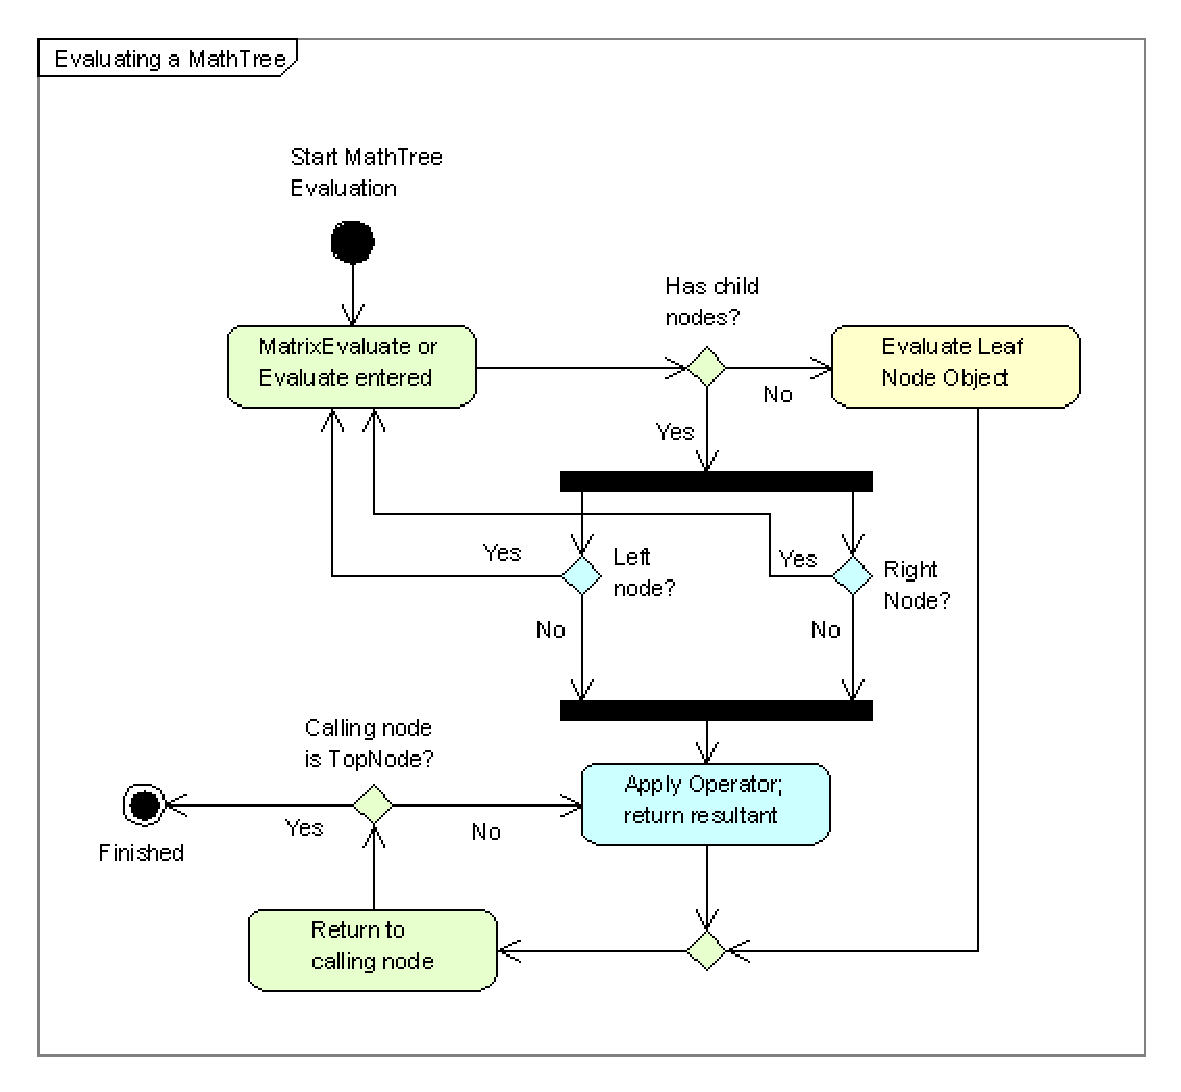
\includegraphics[scale=0.5]{Images/UmlActivitySample.eps}
\caption{\label{figure:UmlActivityExample}An Activity Diagram}
\end{center}
\end{figure}

Activity Diagrams are used to illustrate the work flow for a given task, particularly when the steps
taken in the task can occur in parallel, and when the order of these steps is not necessarily fixed.
 An example of this type of diagram is shown in Figure~\ref{figure:UmlActivityExample}.  This
diagram, which is a subset of the activity diagram shown in Figure~\ref{figure:MathTreeExecution},
shows the actions that occur when an equation is evaluated in a MathTree object.

Action starts at the black circle, in this case in the upper left of the figure, and follows the
arrows through the blocks on the figure, terminating when it reaches the other circular marker, a
filled circle with a concentric circle around it.  Each rounded block in the diagram represents a
step in the task, referred to as an activity in the UML documentation.  These blocks include text
indicating the activity to be accomplished.

Diamond shaped markers are used to indicate splits in the control flow through the diagram.  There
are two types markers used for this purpose: branches, which have a single input with multiple
exits, and merges, which bring together multiple paths to a single output.  Text labels are placed
on the branch markers indicating the test that is performed for the branching.  Labels on each
branch indicate which path is followed based on the test.  For example, in the figure, the branch
point labeled ``Has child nodes?'' proceeds downwards if the current node has child nodes, and to
the right if the current node does not have child nodes.

Activity diagrams also have fork nodes, which are displayed as heavy, black horizontal line
segments.  Fork nodes are used to split the work flow into parallel paths that are all executed. 
The example in the figure shows the evaluation of the subnodes nodes of a MathNode object.  Each
MathNode operator can have a left subnode and a right subnode.  These subnodes must be evaluated
before the operator can execute, but it does not matter which subnode is evaluated first, as long as
the results of both are available when the operator is applied.  The diagram indicates this behavior
by forking the process into parallel paths, and then showing the process logic for each of these
paths.  When both lines of execution complete, the work flow comes back together into a single
execution path.  This merging of the control paths is shown by a second heavy black line segment,
called a Join Node in the UML specifications.

\section{State Diagrams}

\begin{figure}[htb]
\begin{center}
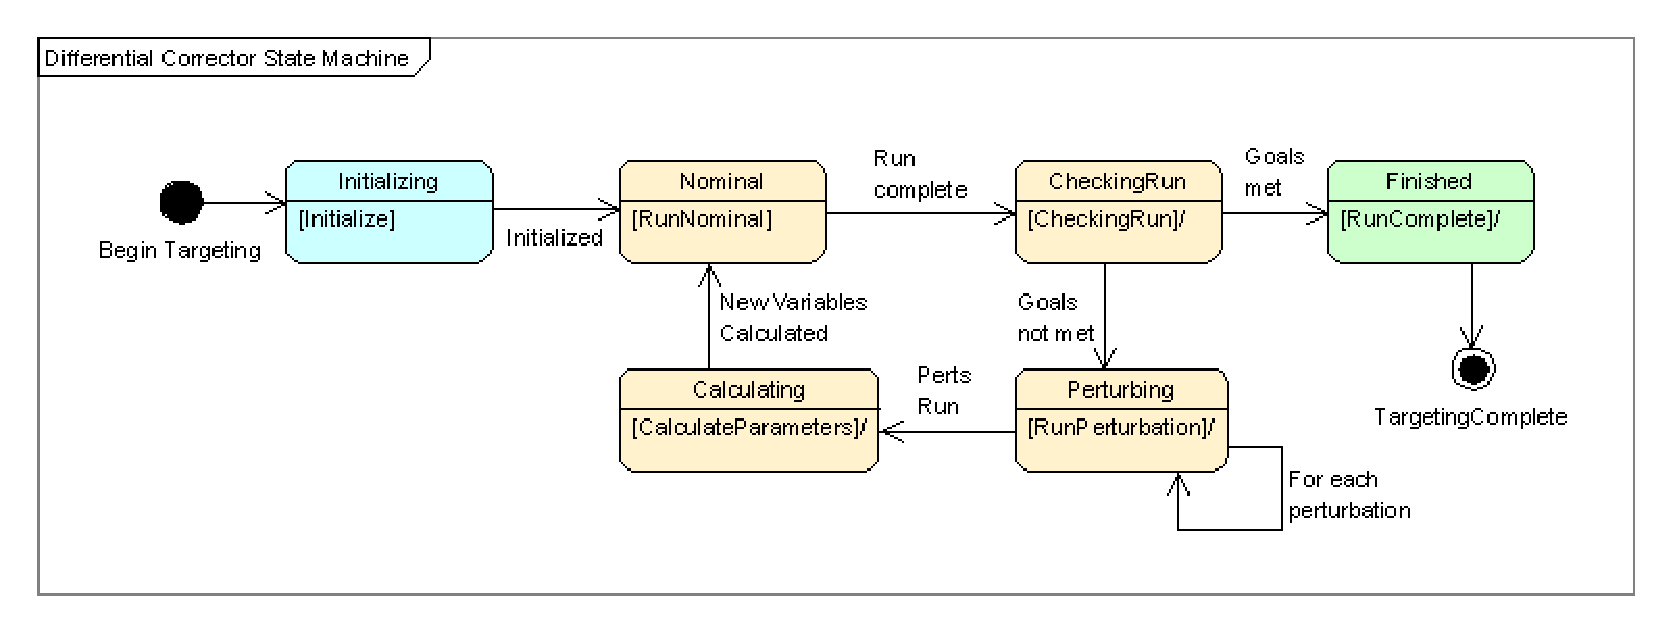
\includegraphics[scale=0.5]{Images/UmlStateSample.eps}
\caption{\label{figure:UmlStateExample}A State Diagram}
\end{center}
\end{figure}

State diagrams are similar in format to activity diagrams.  The start and end nodes are marked the
same way as in an activity diagram, and the program flow is shown using similar transition arrows. 
The differences lie in the objects represented by the diagram, and interpretation of the figure. 
Activity diagrams are used to illustrate the interactions amongst various objects that collectively
perform a task.  State diagrams are used to model how a specific component evolves over time.

In this model of the component being described, that component is always modeled as being in a
specific system state, and transitioning from that state to another state based on changes in the
system.  The Solvers in GMAT are implemented explicitly as finite state machines, so they provide a
prime example for this type of diagram; the finite state machine for a differential corrector object
is shown in Figure~\ref{figure:UmlStateExample}.

Each block in a state diagram represents one of the states available for the object.  These blocks
are divided into two sections.  The upper portion of the block provides a label for the state.  The
lower portion of the block provides information about the process executed within that block -- in
this case, the method called on the object -- and may also provide information about the outcome of
that process.  For the differential corrector shown here, the states are Initializing, Nominal,
CheckingRun, Perturbing, Calculating, and Finished.  Each of these states includes the descriptor
for the function called when the state machine is executed.

The arrows connecting the blocks in this figure show the allowed state transitions.  Each arrow is
labeled with the check that is made to ensure that it is time to make the corresponding transition.
